\tikzset{
    partial ellipse/.style args={#1:#2:#3}{
        insert path={+ (#1:#3) arc (#1:#2:#3)}
    }
}
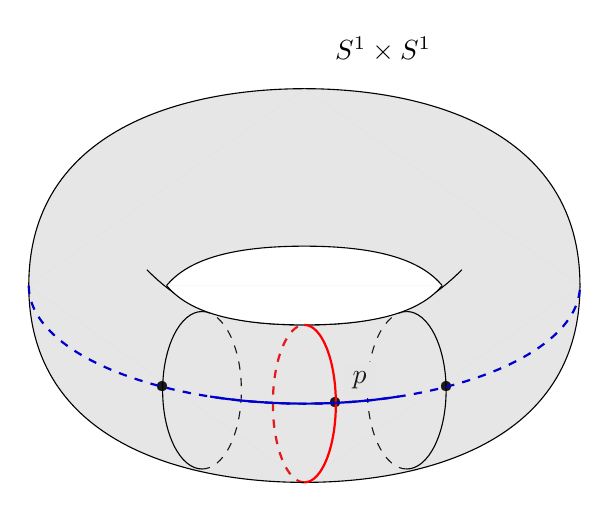
\begin{tikzpicture}

   \draw[dashed] (1.3,-1.33) [partial ellipse= 90:270:0.5cm and 1cm];
   \draw[dashed] (-1.3,-1.33) [partial ellipse=90:-90:0.5cm and 1cm];
   \draw[thick, red,dashed] (-0,-1.5) [partial ellipse=270:90:0.4cm and 1cm];
   \node[fill=white] at (0.7,-1.2) {$p$};
  \node at (0.4,-1.5){\textbullet};
   \node at (1.8,-1.3){\textbullet};
   \node at (-1.8,-1.3){\textbullet};
\fill[fill=gray,fill opacity = 0.2]  (-3.5,0) -- (0, 2.5)  -- (3.5,0);
\fill[fill=gray,fill opacity = 0.2]  (-3.5,0) -- (0, -2.5)  -- (3.5,0);
\draw[fill=gray,fill opacity = 0.2] (-3.5,0) .. controls (-3.5,2) and (-1.5,2.5) .. (0,2.5);
\draw[xscale=-1,fill=gray,fill opacity = 0.2] (-3.5,0) .. controls (-3.5,2) and (-1.5,2.5) .. (0,2.5);
\draw[rotate=180,fill=gray,fill opacity = 0.2] (-3.5,0) .. controls (-3.5,2) and (-1.5,2.5) .. (0,2.5);
\draw[yscale=-1,fill=gray,fill opacity = 0.2] (-3.5,0) .. controls (-3.5,2) and (-1.5,2.5) .. (0,2.5);

\draw (-2,.2) .. controls (-1.5,-0.3) and (-1,-0.5) .. (0,-.5) .. controls (1,-0.5) and (1.5,-0.3) .. (2,0.2);

\draw[fill=white] (-1.75,0) .. controls (-1.5,0.3) and (-1,0.5) .. (0,.5) .. controls (1,0.5) and (1.5,0.3) .. (1.75,0);
\draw[fill=white] (-1.75,0) .. controls (-1.5,-0.3) and (-1,-0.5) .. (0,-.5) .. controls (1,-0.5) and (1.5,-0.3) .. (1.75,0);
  \draw[thick, red] (-0,-1.5) [partial ellipse=90:-90:0.4cm and 1cm];
   \draw (1.3,-1.33) [partial ellipse=90:-90:0.5cm and 1.cm];

    \draw (-1.3,-1.33)  [partial ellipse=270:90:0.5cm and 1cm];
    
    \draw[dashed,  blue!80!black,thick] (-0,0) [partial ellipse=-180:0:3.5cm and 1.5cm];
    \draw[thick,  blue!80!black] (-0,0) [partial ellipse=-110:-70:3.5cm and 1.5cm];
  \node at (1,3) {$\mathbb{S}^1\times\mathbb{S}^1$};
\end{tikzpicture}
